\documentclass[UTF8,8pt]{ctexart}
\usepackage{../template/Notes/notes}
\usepackage{multicol}
\usepackage{pdfpages}
\setlength{\premulticols}{1pt}
\setlength{\postmulticols}{1pt}
\setlength{\multicolsep}{1pt}
\setlength{\columnsep}{2pt}
\setcounter{secnumdepth}{0}
% Redefine section commands to use less space
\makeatletter
\renewcommand{\section}{\@startsection{section}{1}{0mm}%
    {-1ex plus -.5ex minus -.2ex}%
    {0.5ex plus .2ex}%x
{\normalfont\large\bfseries}}
\renewcommand{\subsection}{\@startsection{subsection}{2}{0mm}%
    {-1ex plus -.5ex minus -.2ex}%
    {0.5ex plus .2ex}%
{\normalfont\normalsize\bfseries}}
\renewcommand{\subsubsection}{\@startsection{subsubsection}{3}{0mm}%
    {-1ex plus -.5ex minus -.2ex}%
    {1ex plus .2ex}%
{\normalfont\small\bfseries}}
\makeatother
\setlength{\parindent}{0pt}
\setlength{\parskip}{0pt plus 0.4ex}
\geometry{left=0.1cm,right=0.1cm,top=0.1cm,bottom=0.2cm}
\title{ED Cheatsheet}
\begin{document} 
\leftmargini=5mm
\raggedright
\footnotesize
\begin{multicols}{3}
\se{方程}
    真空麦克斯韦方程 
    $$\ar{
        \nabla\cdot\bm{E} \x  \f{\rho}{\epsilon_0}& \oint_S\bm{E}\d \bm{s} \x  \f{Q}{\epsilon_0}\\
        \nabla\cdot\bm{B} \x  0&\oint_S\bm{B}\d \bm{s} \x  0\\
        \nabla\times\bm{E} \x  -\pt{\bm{B}}& \oint_L\bm{E}\d \bm{l} \x  -\dt{\varphi_B}\\
        \nabla\times\bm{B} \x  \mu_0\bm{J}+\mu_0\epsilon_0 \pt{\bm{E}}& \oint_L\bm{B}\d \bm{l} \x  \mu_0I+\mu_0\epsilon_0\dt{\varphi_E}
    }$$
    
    物质内麦克斯韦方程
    $$\ar{
        \nabla\cdot\bm{D} \x  \rho_f& \oint_S\bm{D}\d \bm{s} \x  Q_f\\
        \nabla\cdot\bm{B} \x  0& \oint_S\bm{B}\d \bm{s} \x  0\\
        \nabla\times\bm{E} \x  -\pt{\bm{B}}&\quad \oint_L\bm{E}\d \bm{l} \x  -\dt{\varphi_B}\\
        \nabla\times\bm{H} \x  \bm{J}_f+\pt{\bm{D}}& \oint_L\bm{H}\d \bm{l} \x  I_f+\dt{\varphi_D}
    }$$
    格林函数法
    $\nabla^2G(x,x')=-\ff{\ep}\de^3(x-x')$\\
    给定$\rho(x')$, 第一类边值问题的解为($G$交换了$x,x'$):\\
    $\vp(x)=\int_VG(x',x)\rho(x')\d V'+\ep_0\oint_S(G(x',x)\pp{\vp}{n'}-\vp(x')\pp{G(x',x)}{n'}\d S')$\\
    若给定边界$\vp$, 则应使$G$在边界为0, 若给定边界$\pp{\vp}{n}$, 则应使$\pp{G}{n}$在边界为0.\\
    电多极矩\\
    $\varphi(\bm{x})=\frac{1}{4 \pi \epsilon_{0}}(\frac{q}{R}+\f{\bm{p}\cdot\bm{R}}{R^3} + \frac{1}{6} \sum_{i, j} \mathfrak{D}_{i j} \frac{\partial^{2}}{\partial x_{i} \partial x_{j}} \frac{1}{R}+\cdots)$\\
    $\bm{E}=-\ca(\f{3(\bm{p}\cdot\bm{R})\bm{R}}{R^5}-\f{\bm{p}}{R^3})$\\
    $\bm{p}=\iiint_V\rho(x')x'\d^3x'$\\
    $\mathfrak{D}=\iiint_{V} 3 \bm{x}^{\prime} \bm{x}^{\prime} \rho(\bm{x}^{\prime}) d^{3} x^{\prime}$\\
    磁偶极矩
    $$\vp = \f{\bm{m}\cdot\bm{R}}{4\pi R^3}, \bm{m}=\ff{2}\iiint_V\bm{x}'\tm \bm{J}(\bm{x'})\d^3x'$$

    边界条件
    $$\ar{
        \text{磁场}&&&\text{电场}\\
        \hline
        \varphi_{1} \x  \varphi_{2}&\varphi_{1} \x  \varphi_{2} \\ 
        \mu_{1} \frac{\partial \varphi_{1}}{\partial n}  \x   \mu_{2} \frac{\partial \varphi_{2}}{\partial n} & \varepsilon_{1} \frac{\partial \varphi_{1}}{\partial n}+\sg_f \x  \varepsilon_{2} \frac{\partial \varphi_{2}}{\partial n}\\
        &&\sg_{\text{电导}1}\frac{\partial \varphi_{1}}{\partial n} \x  \sg_{\text{电导}2}\frac{\partial \varphi_{2}}{\partial n}\\
        H_{1\parallel}+\bm{\a}_f \x  H_{2\parallel}&E_{1\parallel} \x  E_{2\parallel}\\  
        B_{1\perp} \x  B_{2\perp}&D_{1\perp}+\sg_f \x  D_{2\perp}\\
        M_{1\perp}+\a_M  \x   M_{2\perp} & \\
        B_\perp  \x   0 (\text{超导球}) & D_\perp  \x   \sg_f (\text{导体})
    }$$
    
    洛伦兹力:$\bm{f}=\rho\bm{E}+\bm{J}\times\bm{B}$
    
    磁偶极子:$\vec{B}=\frac{\mu_{0}}{4 \pi} \frac{3(\vec{m} \cdot \widehat{R}) \widehat{R}-\vec{m}}{R^{3}}$, $\vp = \f{\bm{m}\cdot\bm{R}}{4\pi R^3}$. 
    
    电磁场:$\bm{S}=\bm{E}\times\bm{H}$, $w=\ff{2}(\bm{E\cdot D}+\bm{H\cdot B})=\ff{2}(\rho\vp+\bm{J}_f\cdot\bm{A})$. 
    
    电流:
    $$\nabla\cdot J=-\pt{\rho},J=\sigma E$$
    
    毕奥——萨伐尔定律  $\bm{B}=\frac{\mu_0}{4\pi}\int\frac{I\d l\times \bm{e}_r}{r^2}$,若$I$为直线,$B=\f{\mu_0Il}{4\pi r^2}$.
    
    
    磁矢势:\\
    库仑规范:
    $$\ar{
        \bm{\nabla}\cdot \bm{A} \x 0
    }$$
    洛伦兹规范:
    $$  \bm{\nabla}\cdot\bm{A}+\ff{c^2}\pt{\varphi} = 0$$
    达朗贝尔方程:
    $$\square \varphi = -\f{\rho}{\epsilon_0},\bm{\square A} = -\mu_0\bm{J}$$
    \sub{超导体}
    临界磁场: 超过$H_c(T)=H_c(0)\left[1-\of{\f{T}{T_c}}^2\right]$时, 超导电性会被破坏. \\
    迈斯纳效应: 超导体内部$B=0$. \\
    伦敦第一方程
    $$\pp{J_s}{t}=\a E,\a=\f{n_se^2}{m}$$
    伦敦第二方程
    $$\nabla\tm\bm{J_s}=-\a B$$
    \se{电磁波的传播}
$\ar{
    \bm{\nabla}\times \bm{B}-\ff{c^2}\pt{\bm{E}} \x  0\quad&\quad \bm{\nabla^2 E}-\ff{c^2}\pt[2]{\bm{E}}=\square \bm{E} \x  0\\
    \bm{\nabla}\times \bm{E}+\pt{\bm{B}} \x  0&\bm{\nabla^2 B}-\ff{c^2}\pt[2]{\bm{B}}=\square \bm{B} \x  0
}$
    $$\abs{\f{E}{B}}=\ff{\sqrt{\mu\ep}}=v$$
    $$S=\sqrt{\f{\ep}{\mu}}E^2\bm{e}_k=vw\bm{e}_k$$
    群速与相速关系
    $$v_g=\dd{\o}{k}=v_p+k\dd{v_p}{k}=\f{c}{n+\o(\d n/\d\o)}$$
    导体内波矢量$k=\b+i\a,v\o/\b$. 垂直入射时$\a\approx\b\approx\sqrt{\o\mu\sg/2}, B\approx \sqrt{\mu\sg/\o}e^{i\f{\pi}{4}}e_n\tm E$. B的相位比E滞后1/4. 金属内部主要是磁场能. 电磁波穿透深度为$\de=\ff{\a}=\sqrt{2/\o\mu\sg}$, 此为趋肤效应. 
    \sub{反射}
    介质界面上的边界条件为
    $$\ar{
        e_n\tm(E_2-E_2)\x0\\
        e_n\tm(H_2-H_1)\x\a
    }$$
    入射波, 反射波和折射波分别为$E,E',E''$. 从介质1射向介质2. 有边界条件$\bm{k\cdot x}=\bm{k'\cdot x}=\bm{k''\cdot x}$\\
    菲涅耳公式:\\
    当$E\perp$入射面(s光):
    \begin{equation}
        \f{E'}{E} = \f{\sqrt{\ep_1}\cos\t-\sqrt{\ep_2}\cos\t''}{\sqrt{\ep_1}\cos\t+\sqrt{\ep_2}\cos\t''}=-\f{\sin(\t-\t'')}{\sin(\t+\t'')}
    \end{equation}
    \begin{equation}
        \f{E''}{E} = \f{2\sqrt{\ep_1}\cos\t}{\sqrt{\ep_1}\cos\t+\sqrt{\ep_2}\cos\t''}=\f{2\cos\t\sin\t''}{\sin(\t+\t'')}
    \end{equation}
    当$E\parallel$入射面(p光):
    $$\ar{
        \f{E'}{E}\x \f{\tan(\t-\t'')}{\tan(\t+\t'')}\\
        \f{E''}{E}\x \f{2\cos\t\sin\t''}{\sin(\t+\t'')\cos(\t-\t'')}
    }$$
    布儒斯特角: 当$\t+\t''=90^\circ$, $E_\parallel'$消失. $\tan\t_B=n_{21}$\\
    半波损失: 前一种情况反射波与入射波反相. \\
    反射系数和透射系数
    $$R=\f{E_0'^2}{E_0^2}, T=\f{n_2\cos\t''}{n_1\cos\t}\f{E_0''^2}{E_0^2}$$
    $$R_s=(1)^2,R_p=(2)^2$$
    $$T_s=\f{\sin2\t\sin2\t''}{\sin^2(\t+\t'')},T_p=\f{4\sin2\t\sin2\t''}{(\sin2\t+\sin2\t'')^2}$$
    当$\t=0$, $R_s=R_p=\f{(n_2-n_1)^2}{(n_2+n_1)^2}$. \\
    全反射:$k_z''=i\kappa,\ \kappa=k\sqrt{\sin^2\t-n_{21}^2}$\\
    全反射能量守恒为:$R+\f{\cos\t''}{\cos\t}T=1$\\
    垂直入射到良导体($\f{\sg}{\o\ep}>>1$)表面:
    $$R=1-2\sqrt{\f{2\o\ep_0}{\sg}}=\f{(n-n_1)^2+\kappa}{(n+n_1)+\kappa^2}$$
    $$\ep'=\ep+i\f{\sg}{\o}$$
    折射波场沿x轴传播, 场强沿z轴指数衰减:
    $$\bm{E}''=\bm{E}''_0e^{-\kappa z}e^{i(k''_xx-\o t)}$$
    其厚度$\sim\kappa^{-1}=\ff{\l_1}{2\pi\sqrt{\sin^2\t-n_{21}^2}}$
    \sub{矩形谐振腔}
    1代表导体, 2代表真空. 法线由导体指向介质. 满足亥姆霍兹方程$\nabla^2u+k^2u=0$. 边界条件为$E_\parallel=H_\perp=\pp{E_n}{n}=0$.$k=\o\sqrt{\mu\ep}$. \\
    满足$k_xA_1+k_yA_2+k_zA_3=0$. 本征频率$\o=\f{\pi}{\sqrt{\mu\ep}}\sqrt{(m/l_1)^2+\cdots}$. 
    $$\hua{
        E_x \x A_1\cos k_xx \sin k_y y \sin k_zze^{-i\o t}\\
        E_y \x A_2\sin k_xx \cos k_y y \sin k_zze^{-i\o t}\\
        E_z \x A_3\sin k_xx \sin k_y y \cos k_zze^{-i\o t}
    }$$
    $$k_x=\f{m\pi}{l_1},k_y=\f{n\pi}{l_2},k_z=\f{p\pi}{l_3}$$
    \sub{矩形波导}
    $z$方向无穷长的解为$k_x^2+k_y^2+k_z^2=k^2$.$k_xA_1+k_yA_2-ik_zA_3=0$. 
    $$\hua{
        E_x \x A_1\cos k_xx \sin k_y y e^{-k_zz}\\
        E_y \x A_2\sin k_xx \cos k_y y e^{-k_zz}\\
        E_z \x A_3\sin k_xx \sin k_y y e^{-k_zz}
    },\ k_x=\f{m\pi}{a},k_y=\f{n\pi}{b}$$
    $$H=-\f{i}{\o\mu}\nabla\tm E$$
    由上式, $E_z=0$则$H_z\neq 0$. 因此波导中的波不能是TEM. 由于$k_z=\sqrt{(\o/c)^2-(k_x^2+k_y^2)}$为实数, 截止频率为$\o=\pi c\sqrt{(m/a)^2+(n/b)^2}$. 相速度<c, 群速度>c.
    \sub{等离子体}
    振荡频率$\o_p=\sqrt{n_0e^2/m\ep_0}$. $m\ddot{r}=-eE=eE_0e^{i(kx-\o t)}$. $J(\o)=-n_0ev=\sg(\o)E,\sg=i\f{n_0e^2}{m\o}$. 稀薄等离子折射率为$n=\sqrt{1-\o_p^2/\o^2}$. 当$\o>\o_p$,$v_p>c$全反射,可传播电磁波. 
    \sub{推迟势}
    以$R$表示原点$x'$到场点$x$的距离. $r\approx R-e_R\cdot x'$. 
    $$\vp(x,t)=\int_V\f{\r\of{x',t-\f{r}{c}}}{4\pi\ep_0r}\d V'$$
    $A(x,t)=\f{\mu_0}{4\pi}\int_V\f{\bm{J}\of{x',t-\f{r}{c}}}{r}\d V'=\f{\mu_0}{4\pi}\int_V\f{\bm{J}(x')e^{ik(R-e_R\cdot x')}}{R-e_R\cdot x'}\d V'$\\
    展开第一项为:
    $$A(x)=\f{\mu_0e^{ikR}}{4\pi R}\int_VJ(x')\d V'=\f{\mu_0e^{ikR}}{4\pi R}\dot{\bm{p}}$$
    可得电偶极辐射:
    $\hua{
        \bm{B}\x\ff{4\pi\ep_0c^3R}\ddot{p}e^{ikR}\sin\t \bm{e}_\vp\\
        \bm{E}\x\ff{4\pi\ep_0c^3R}\ddot{p}e^{ikR}\sin\t \bm{e}_\t\\
        \bar{\bm{S}} \x \f{|\ddot{p}|^2}{32\pi^2\ep_0c^3R^2}\sin^2\t\bm{e}_R\\
        P \x \oint|\bar{\bm{S}}|R^2\d\O = \ff{4\pi\ep_0}\f{|\ddot{p}|^2}{3c^3}
    }$\\
    磁偶极辐射和电四极辐射
    展开第二项:($\mathcal{D}=\sum 3qx'_ix'_j-r'^2\de_{ij}$)\\
    $A(x)=\f{-ik\mu_0e^{ikR}}{4\pi R}\int_V\bm{J}(x')(\bm{e_R\cdot x'}\d V')=\f{-ik\mu_0e^{ikR}}{4\pi R}\of{-\bm{e_R\tm m}+\ff{6}\bm{e_R}\cdot\dot{\mathcal{D}}}$\\
    先计算磁偶极辐射$A=\f{ik\mu_0e^{ikR}}{4\pi R}\bm{e_R\tm m}$.
    $$\hua{
        \bm{B} \x \f{\mu_0e^{ikR}}{4\pi c^2R}(\ddot{m}\tm e_R)e_R\\
        \bm{E} \x -\f{\mu_0e^{ikR}}{4\pi cR}(\ddot{m}\tm e_R)\\
        \bm{\bar{S}} \x \f{\mu_0\o^4|\bm{m}|^2}{32\pi^2c^3R^2}\sin^2\t e_R\\
        P\x \f{\mu_0\o^4|\bm{m}|^2}{12\pi c^3}
    }$$
    再计算电四极辐射$A=\f{-ik\mu_0e^{ikR}}{24\pi R}\dot{\mathcal{D}}$. 定义$\bm{D}=e_R\cdot \mathcal{D}$. 
    $$\hua{
        A(x) \x \f{e^{ikR}}{24\pi\ep_0c^4R}\dddot{\bm{D}}\tm e_R\\
        B \x ik\bm{e_R\tm A}\\
        E \x c\bm{B\tm{e_R}}\\
        S \x \ff{4\pi\ep_0}\ff{288\pi c^5R^2}(\dddot{\bm{D}}\tm e_R)^2e_R
    }$$
    \sub{衍射}
    基尔霍夫公式:$\psi(x)=-\ff{4\pi}\oint_S\f{e^{ikr}}{r}\bm{e}_n\cdot\left[\nabla'\psi+\of{ik-\ff{r}}\f{\bm{r}}{r}\psi\right]\d S'$.\\
    夫琅禾费衍射: $x'$为小孔上一点, $x$为空间远处一点, $R$为小孔中心到远处距离. $k_1$沿入射方向, $k_2$沿R方向. $\t_1,\t_2$为入射出射角. 
    $$\phi(x)=-\f{i\psi_0e^{ikR}}{4\pi R}\int_{S}e^{i(k_1-k_2)\cdot x'}(\cos\t_1+\cos\t_2)\d S'$$
    长宽为$\a,\b$的矩形孔夫琅禾费衍射为:
    $$I=I_0\of{\f{1+\cos\t_2}{2}}^2\of{\f{\sin ka\a}{ka\a}}^2\of{\f{\sin kb\b}{kb\b}}^2$$
    电磁场动量:\\
    动量密度$\bm{g}=\ep_0\bm{E\tm B}=\ff{c^2}\bm{S}=\f{w}{c}\bm{e}_k$. 
    \se{狭义相对论}
    $
    a=\left(\begin{smallmatrix}{\gamma} & {0} & {0} & {i \beta \gamma} \\ {0} & {1} & {0} & {0} \\ {0} & {0} & {1} & {0} \\ {-i \beta \gamma} & {0} & {0} & {\gamma}\end{smallmatrix}\right),\quad\beta=\frac{v}{c}, \quad \gamma=\frac{1}{\sqrt{1-\beta^{2}}}
     $\\
    定义固有时$d \tau=\frac{1}{c} d s$和4-速度:$U_{\mu}=\frac{d x_{\mu}}{d \tau}=\gamma_{u}\left(u_{1}, u_{2}, u_{3}, i c\right)$. \\
    相对论多普勒效应
    $
    \omega \approx \frac{\omega_{0}}{1-\frac{v}{c} \cos \theta}
     $\\
    定义场强张量
    $
    F_{\mu \nu}=\left[\begin{smallmatrix}{cccc}{0} & {B_{3}} & {-B_{2}} & {-\frac{1}{c} E_{1}} \\ {-B_{3}} & {0} & {B_{1}} & {-\frac{\mathbf{i}}{c} E_{2}} \\ {B_{2}} & {-B_{1}} & {0} & {-\frac{\mathbf{i}}{c} E_{3}} \\ {\frac{\mathbf{i}}{c} E_{1}} & {\frac{\mathbf{i}}{\boldsymbol{c}} \boldsymbol{E}_{2}} & {\frac{\mathbf{i}}{c} \boldsymbol{E}_{3}} & {0}\end{smallmatrix}\right]
     $\\
     Maxwell方程变为
     $
    \frac{\partial F_{\mu v}}{\partial x_{v}}=\mu_{0} J_{\mu}
     $,
     $
    \frac{\partial F_{\mu \nu}}{\partial x_{\lambda}}+\frac{\partial F_{v \lambda}}{\partial x_{\mu}}+\frac{\partial F_{\lambda \mu}}{\partial x_{v}}=0
     $\\
     且满足
     $$ 
    \begin{aligned} \frac{1}{2} F_{\mu \nu} F_{\mu \nu}=B^{2} &-\frac{1}{c^{2}} E^{2} \\ \frac{i}{8} \epsilon_{\mu \nu \lambda \tau} F_{\mu \nu} F_{\lambda \tau}=& \frac{1}{c} \vec{B} \cdot \vec{E} \end{aligned}
     $$
    能动量洛伦兹变换
    $$ 
    \begin{array}{l}{p_{1}=\frac{p_{1}^{\prime}+\frac{\beta_{c}}{c^{2}} E_{1}^{\prime}}{\sqrt{1-\beta_{c}^{2} / c^{2}}} ; E_{1}=\frac{E_{1}^{\prime}+\beta_{c} p_{1}^{\prime}}{\sqrt{1-\beta_{c}^{2} / c^{2}}}} \\ {p_{2}=\frac{p_{2}^{\prime}+\frac{\beta_{c}}{c^{2}} E_{2}^{\prime}}{\sqrt{1-\beta_{c}^{2} / c^{2}}} ;E_{2}=\frac{E_{2}^{\prime}+\beta_{c} p_{2}^{\prime}}{\sqrt{1-\beta_{c}^{2} / c^{2}}}}\end{array}
     $$
    \se{数学}
    \sub{柱坐标系 $(\rho,\phi,z)$}
    $\nabla \varphi = \hat e_1 \frac { \partial \varphi } { \partial \rho } + \hat e_2 \frac { 1 } { \rho } \frac { \partial \varphi } { \partial \phi } + \hat { e } _ { 3 } \frac { \partial \varphi } { \partial z }$
    $\nabla \cdot \bm{ A } = \frac { 1 } { \rho } \frac { \partial ( \rho A _ { 1 } ) } { \partial \rho } + \frac { 1 } { \rho } \frac { \partial A _ { 2 } } { \partial \phi } + \frac { \partial A _ { 3 } } { \partial z }$
    $ { \nabla \times \bm{ A } } =\hat e_1 (\ff{\rho} \frac { \partial A_3} { \partial \phi } - \frac { \partial A _ { 2 } } { \partial z } ) + \hat { e } _ { 2 } ( \frac { \partial A _ { 1 } } { \partial z } - \frac { \partial A _ { 3 } } { \partial \rho } ) + \hat { e } _ { 3 } \frac { 1 } { \rho } ( \frac { \partial ( \rho A _ { 2 } ) } { \partial \rho } - \frac { \partial A _ { 1 } } { \partial \phi } )$
    $\nabla ^ { 2 } \varphi = \frac { 1 } { \rho } \frac { \partial } { \partial \rho } ( \rho \frac { \partial \varphi } { \partial \rho } ) + \frac { 1 } { \rho ^ { 2 } } \frac { \partial ^ { 2 } \varphi } { \partial \phi ^ { 2 } } + \frac { \partial ^ { 2 } \varphi } { \partial z ^ { 2 } }$
    \sub{球坐标系 $(r,\t,\varphi)$ }
    $\nabla \varphi = \hat { e } _ { 1 } \frac { \partial \varphi } { \partial r } + \hat { e } _ { 2 } \frac { 1 } { r } \frac { \partial \varphi } { \partial \theta } + \hat { e } _ { 3 } \frac { 1 } { r \sin \theta } \frac { \partial \varphi } { \partial \phi }q$
    $\nabla \cdot \bm{ A } = \ff{r^2} \pp{r^2A_1}{r} + \frac { 1 } { r \sin \theta } \frac { \partial } { \partial \theta } ( \sin \theta A _ { 2 } ) + \frac { 1 } { r \sin \theta } \frac { \partial A _ { 3 } } { \partial \phi }$
    $\nabla \times \bm{ A }  = 
    \hat { e } _ { 1 } \frac { 1 } { r \sin \theta } \left[ \frac { \partial } { \partial \theta } ( \sin \theta A _ { 3 } ) - \frac { \partial A _ { 2 } } { \partial \phi } \right]  
    + \hat { e } _ { 2 } \left[ \frac { 1 } { r \sin \theta } \frac { \partial A _ { 1 } } { \partial \phi } - \frac { 1 } { r } \frac { \partial } { \partial r } ( r A _ { 3 } ) \right] 
    + \hat { e } _ { 3 } \frac { 1 } { r } \left[ \frac { \partial } { \partial r } ( r A _ { 2 } ) - \frac { \partial A _ { 1 } } { \partial \theta } \right] $
    $\nabla^2\varphi=\ff{r^2\sin\t}\left[\sin\t\pp{}{r}(r^2\pp{\varphi}{r})+\pp{}{\t}(\sin\t\pp{\varphi}{\t})+\ff{\sin\t}\pp[2]{\varphi}{\phi}\right]$
    \sub{矢量变换}
    $\nabla\bm{r}=-\nabla'\bm{r}=\bm{e}_r$
    $\nabla\ff{\bm{r}}=-\nabla'\ff{\bm{r}}=-\ff{r^2}\bm{e}_r$
    $\curl\ff{\bm{r}^2}=\div\ff{\bm{r}}=0$
    $\div\vp\bm{A}=\vp\div\bm{A}+\bm{A}\cdot\grad\vp$
    $\curl\vp\bm{A}=\vp\curl\bm{A}+\grad\vp\times\bm{A}$
    $\div(\bm{A}\cdot\bm{B}) = (\bm{A}\cdot\nabla)\bm{B}+(\bm{B}\cdot\nabla)\bm{A}+\bm{A}\tm(\curl\bm{B})+\bm{B}\tm(\curl\bm{A})$
    $\nabla\cdot(\bm{F} \times \bm{G})=(\nabla\times \bm{F})\cdot \bm{G}-\bm{F}\cdot(\nabla\times \bm{G})$
    $\bm{A}\times(\bm{B}\times\bm{C})=(\bm{A}\cdot\bm{C})\bm{B}-(\bm{A}\cdot\bm{B})\bm{C}$
    $( \bm{ A } \times \bm{ B } ) \times ( \bm{ C } \times \bm{ D } ) = [ \bm{ A } \cdot ( \bm{ B } \times \bm{ D } ) ] \bm{ C } - [ \bm{ A } \cdot ( \bm{ B } \times \bm{ C } ) ] \bm{ D }$
    $( \bm{ A } \times \bm{ B } ) \cdot ( \bm{ C } \times \bm{ D } ) = \abs{\ar{\bm{A}\cdot\bm{C}&\ \ \bm{A}\cdot\bm{D}\\
    \bm{B}\cdot\bm{C}&\ \ \bm{B}\cdot\bm{D}}}$
    $\bm{ A } \times ( \bm{ B } \times \bm{ C } ) + \bm{ B } \times ( \bm{ C } \times \bm{ A } ) + \bm{ C } \times ( \bm{ A } \times \bm{ B } ) = 0$
    \end{multicols}
\begin{figure}[htbp]
    \centering
    \begin{minipage}[t]{0.19\linewidth}\centering\boxed{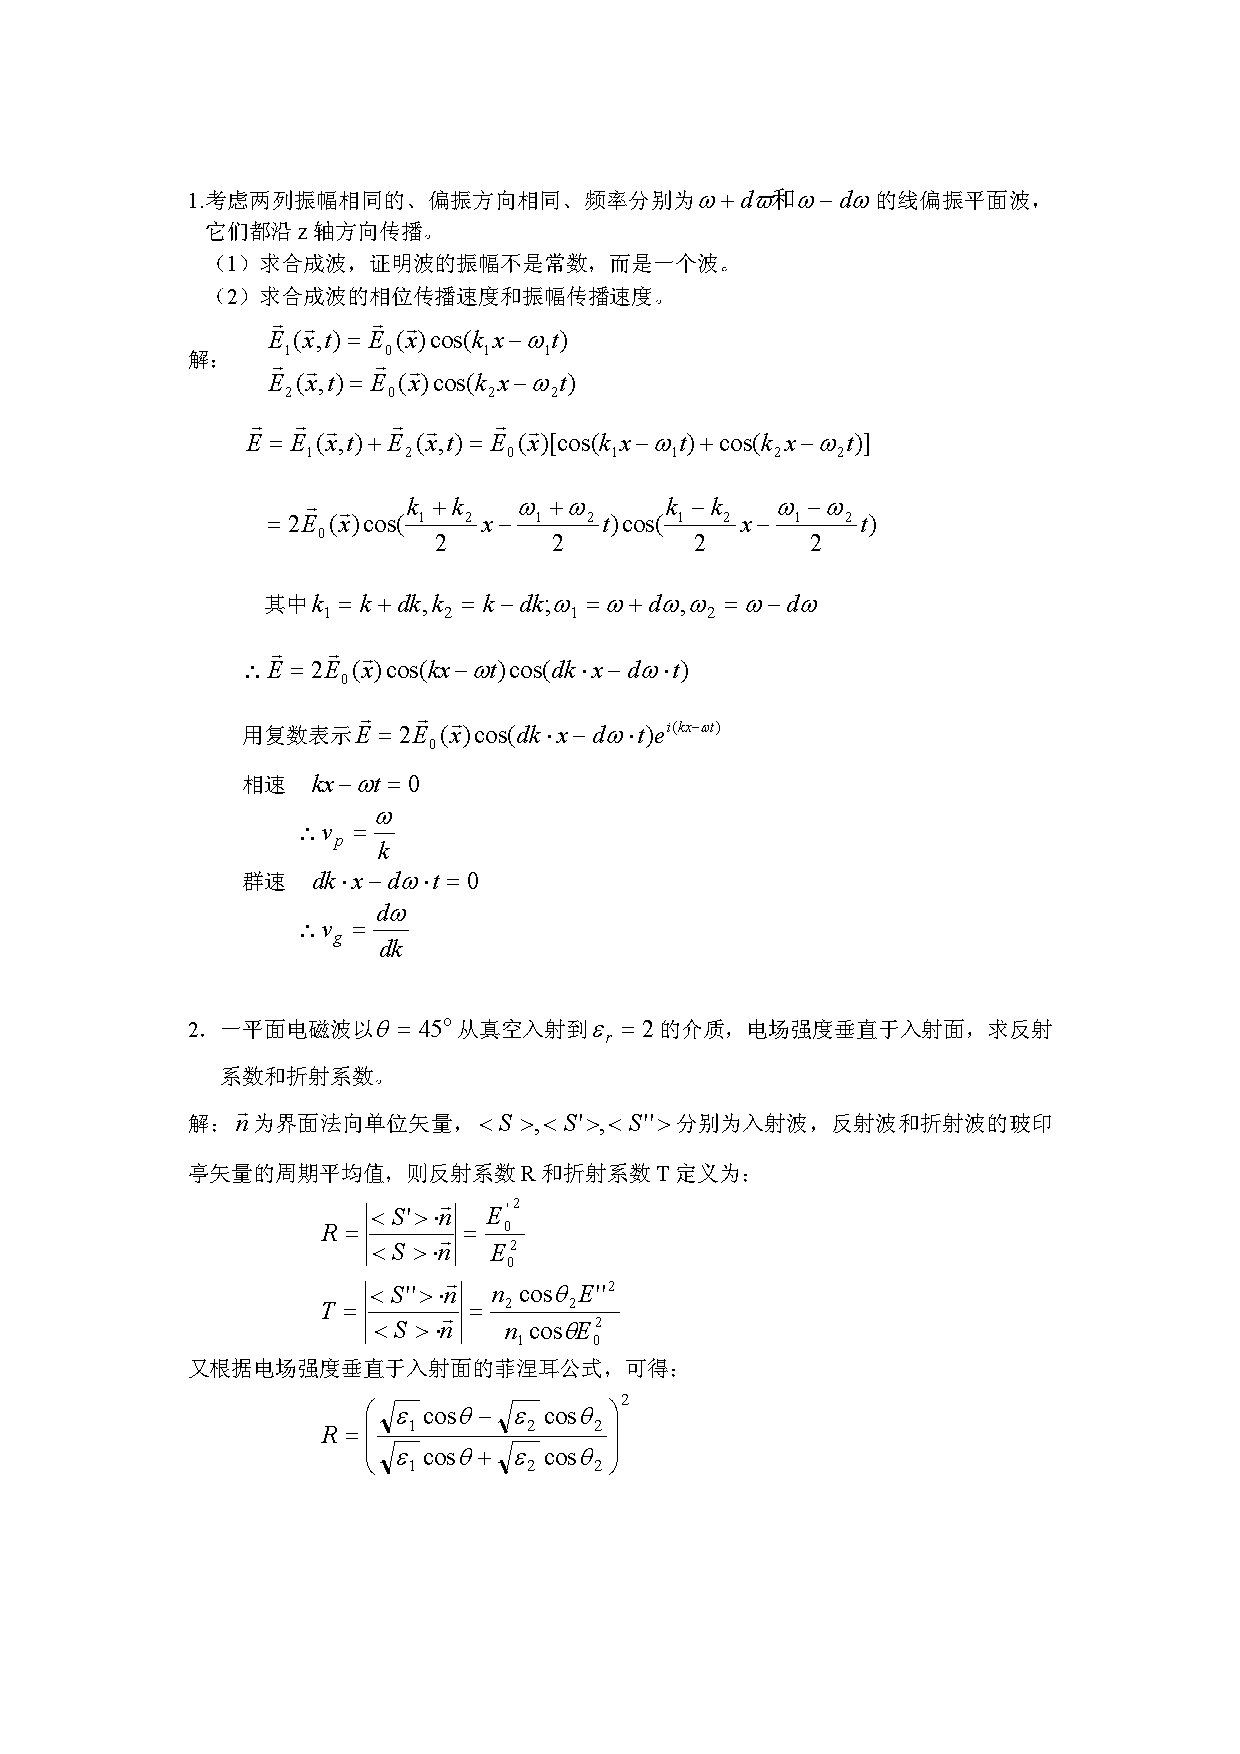
\includegraphics[page=1,width=1\linewidth]{a.pdf}}\end{minipage}
    \begin{minipage}[t]{0.19\linewidth}\centering\boxed{\includegraphics[page=2,width=1\linewidth]{a.pdf}}\end{minipage}
    \begin{minipage}[t]{0.19\linewidth}\centering\boxed{\includegraphics[page=3,width=1\linewidth]{a.pdf}}\end{minipage}
    \begin{minipage}[t]{0.19\linewidth}\centering\boxed{\includegraphics[page=4,width=1\linewidth]{a.pdf}}\end{minipage}
    \begin{minipage}[t]{0.19\linewidth}\centering\boxed{\includegraphics[page=5,width=1\linewidth]{a.pdf}}\end{minipage}
    \begin{minipage}[t]{0.19\linewidth}\centering\boxed{\includegraphics[page=6,width=1\linewidth]{a.pdf}}\end{minipage}
    \begin{minipage}[t]{0.19\linewidth}\centering\boxed{\includegraphics[page=7,width=1\linewidth]{a.pdf}}\end{minipage}
    \begin{minipage}[t]{0.19\linewidth}\centering\boxed{\includegraphics[page=8,width=1\linewidth]{a.pdf}}\end{minipage}
    \begin{minipage}[t]{0.19\linewidth}\centering\boxed{\includegraphics[page=9,width=1\linewidth]{a.pdf}}\end{minipage}
    \begin{minipage}[t]{0.19\linewidth}\centering\boxed{\includegraphics[page=10,width=1\linewidth]{a.pdf}}\end{minipage}
    \end{figure}
    \begin{figure}[htbp]
        \centering
    \begin{minipage}[t]{0.19\linewidth}\centering\boxed{\includegraphics[page=11,width=1\linewidth]{a.pdf}}\end{minipage}
    \begin{minipage}[t]{0.19\linewidth}\centering\boxed{\includegraphics[page=12,width=1\linewidth]{a.pdf}}\end{minipage}
    \begin{minipage}[t]{0.19\linewidth}\centering\boxed{\includegraphics[page=13,width=1\linewidth]{a.pdf}}\end{minipage}
    \begin{minipage}[t]{0.19\linewidth}\centering\boxed{\includegraphics[page=14,width=1\linewidth]{a.pdf}}\end{minipage}
    \begin{minipage}[t]{0.19\linewidth}\centering\boxed{\includegraphics[page=15,width=1\linewidth]{a.pdf}}\end{minipage}
    \begin{minipage}[t]{0.19\linewidth}\centering\boxed{\includegraphics[page=16,width=1\linewidth]{a.pdf}}\end{minipage}
    \begin{minipage}[t]{0.19\linewidth}\centering\boxed{\includegraphics[page=17,width=1\linewidth]{a.pdf}}\end{minipage}
    \begin{minipage}[t]{0.19\linewidth}\centering\boxed{\includegraphics[page=18,width=1\linewidth]{a.pdf}}\end{minipage}
    \begin{minipage}[t]{0.19\linewidth}\centering\boxed{\includegraphics[page=19,width=1\linewidth]{a.pdf}}\end{minipage}
    \begin{minipage}[t]{0.19\linewidth}\centering\boxed{\includegraphics[page=20,width=1\linewidth]{a.pdf}}\end{minipage}
    \begin{minipage}[t]{0.19\linewidth}\centering\boxed{\includegraphics[page=21,width=1\linewidth]{a.pdf}}\end{minipage}
    \begin{minipage}[t]{0.19\linewidth}\centering\boxed{\includegraphics[page=22,width=1\linewidth]{a.pdf}}\end{minipage}
    \begin{minipage}[t]{0.19\linewidth}\centering\boxed{\includegraphics[page=23,width=1\linewidth]{a.pdf}}\end{minipage}
    \begin{minipage}[t]{0.19\linewidth}\centering\boxed{\includegraphics[page=24,width=1\linewidth]{a.pdf}}\end{minipage}
    \begin{minipage}[t]{0.19\linewidth}\centering\boxed{\includegraphics[page=25,width=1\linewidth]{a.pdf}}\end{minipage}
    \begin{minipage}[t]{0.19\linewidth}\centering\boxed{\includegraphics[page=26,width=1\linewidth]{a.pdf}}\end{minipage}
    \begin{minipage}[t]{0.19\linewidth}\centering\boxed{\includegraphics[page=27,width=1\linewidth]{a.pdf}}\end{minipage}
    \begin{minipage}[t]{0.19\linewidth}\centering\boxed{\includegraphics[page=28,width=1\linewidth]{a.pdf}}\end{minipage}
    \begin{minipage}[t]{0.19\linewidth}\centering\boxed{\includegraphics[page=29,width=1\linewidth]{a.pdf}}\end{minipage}
    \begin{minipage}[t]{0.19\linewidth}\centering\boxed{\includegraphics[page=30,width=1\linewidth]{a.pdf}}\end{minipage}
    \end{figure}
    \begin{figure}[htbp]
        \centering
    \begin{minipage}[t]{0.19\linewidth}\centering\boxed{\includegraphics[page=31,width=1\linewidth]{a.pdf}}\end{minipage}
    \begin{minipage}[t]{0.19\linewidth}\centering\boxed{\includegraphics[page=32,width=1\linewidth]{a.pdf}}\end{minipage}
    \begin{minipage}[t]{0.19\linewidth}\centering\boxed{\includegraphics[page=33,width=1\linewidth]{a.pdf}}\end{minipage}
    \begin{minipage}[t]{0.19\linewidth}\centering\boxed{\includegraphics[page=34,width=1\linewidth]{a.pdf}}\end{minipage}
    \begin{minipage}[t]{0.19\linewidth}\centering\boxed{\includegraphics[page=35,width=1\linewidth]{a.pdf}}\end{minipage}
    \begin{minipage}[t]{0.19\linewidth}\centering\boxed{\includegraphics[page=36,width=1\linewidth]{a.pdf}}\end{minipage}
    \begin{minipage}[t]{0.19\linewidth}\centering\boxed{\includegraphics[page=37,width=1\linewidth]{a.pdf}}\end{minipage}
    \begin{minipage}[t]{0.19\linewidth}\centering\boxed{\includegraphics[page=38,width=1\linewidth]{a.pdf}}\end{minipage}
    \begin{minipage}[t]{0.19\linewidth}\centering\boxed{\includegraphics[page=39,width=1\linewidth]{a.pdf}}\end{minipage}
    \begin{minipage}[t]{0.19\linewidth}\centering\boxed{\includegraphics[page=40,width=1\linewidth]{a.pdf}}\end{minipage}
    \begin{minipage}[t]{0.19\linewidth}\centering\boxed{\includegraphics[page=41,width=1\linewidth]{a.pdf}}\end{minipage}
    \begin{minipage}[t]{0.19\linewidth}\centering\boxed{\includegraphics[page=42,width=1\linewidth]{a.pdf}}\end{minipage}
    \begin{minipage}[t]{0.19\linewidth}\centering\boxed{\includegraphics[page=43,width=1\linewidth]{a.pdf}}\end{minipage}
    \begin{minipage}[t]{0.19\linewidth}\centering\boxed{\includegraphics[page=44,width=1\linewidth]{a.pdf}}\end{minipage}
    \begin{minipage}[t]{0.19\linewidth}\centering\boxed{\includegraphics[page=45,width=1\linewidth]{a.pdf}}\end{minipage}
    \begin{minipage}[t]{0.19\linewidth}\centering\boxed{\includegraphics[page=46,width=1\linewidth]{a.pdf}}\end{minipage}
    \begin{minipage}[t]{0.19\linewidth}\centering\boxed{\includegraphics[page=47,width=1\linewidth]{a.pdf}}\end{minipage}
    \begin{minipage}[t]{0.19\linewidth}\centering\boxed{\includegraphics[page=48,width=1\linewidth]{a.pdf}}\end{minipage}
    \begin{minipage}[t]{0.19\linewidth}\centering\boxed{\includegraphics[page=49,width=1\linewidth]{a.pdf}}\end{minipage}
    \begin{minipage}[t]{0.19\linewidth}\centering\boxed{\includegraphics[page=50,width=1\linewidth]{a.pdf}}\end{minipage}
\end{figure}
\end{document}